
\clearpage
\section{Document Management}
\label{bkm:Ref434830029}\label{bkm:Ref434828324}

\begin{wrapfigure}[13]{l}{6.5cm}   % [x] Wie manche Zeile soll sich um die Grafik "brechen"
  \vspace{-35pt}      % Grundwert war 20; mit 30 schön oben beim Text ausgerichtet
  \begin{center}
    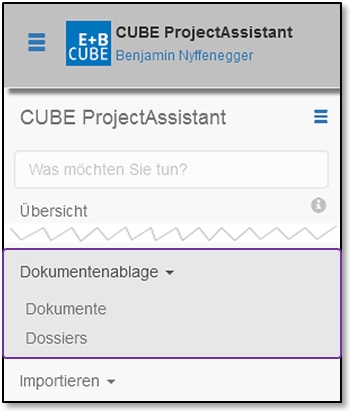
\includegraphics[width=1\linewidth]{../chapters/11_Dokumentenablage/pictures/11_Menu_Dokumentenablage.jpg}
  \end{center}
  \vspace{-20pt}
  \caption{Using the document management}
  \vspace{-10pt}
\end{wrapfigure}

Select the 'Document Management' menu item in the main menu on the left. The subcategories 'Documents' and 'Dossiers' appear.

\vspace{\baselineskip}

The document management function is used to manage documents and to edit them. When documents or their metadata are edited, they receive a new version number in CUBE PA. On one hand, the check-out and check-in functions guarantee that a document is only edited by one user at once. On the other hand, the versioning of documents ensures that all project participants can refer to unique document versions.

\vspace{1cm}  

Entered or uploaded documents can be sorted into dossiers, which can then easily be downloaded. For this reason, creating and handling a dossier are described first in the tutorial.

\vspace{\baselineskip}

Document management will then be explained in detail.

\subsection{Dossiers}
\label{bkm:Ref442544219}\subsubsection{Creating dossiers}

A dossier is a set of related documents. A classic example is a planning approval dossier or a preliminary project. Dossiers enable the grouping together of several uploaded documents, so that they can later be downloaded together in a ZIP archive.

\begin{figure}[H]
\center{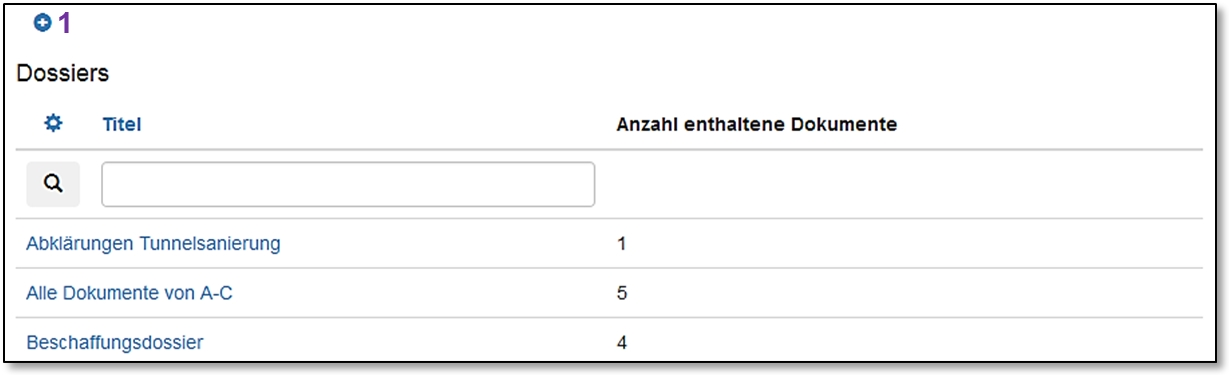
\includegraphics[width=1\linewidth]{../chapters/11_Dokumentenablage/pictures/11-1-1_UebersichtDossiers.jpg}}
\caption{Creating a new dossier}
% \label{fig:speciation}
\end{figure}

To create a new dossier, select the 'Document Management' menu item in the menu on the left then click on 'Dossiers'. Then click on the plus symbol 
\includegraphics[height=12pt]{/Icons/Plussymbol.jpg} \col{(1)}.

\vspace{\baselineskip}

The input form for dossiers appears:

\begin{figure}[H]
\center{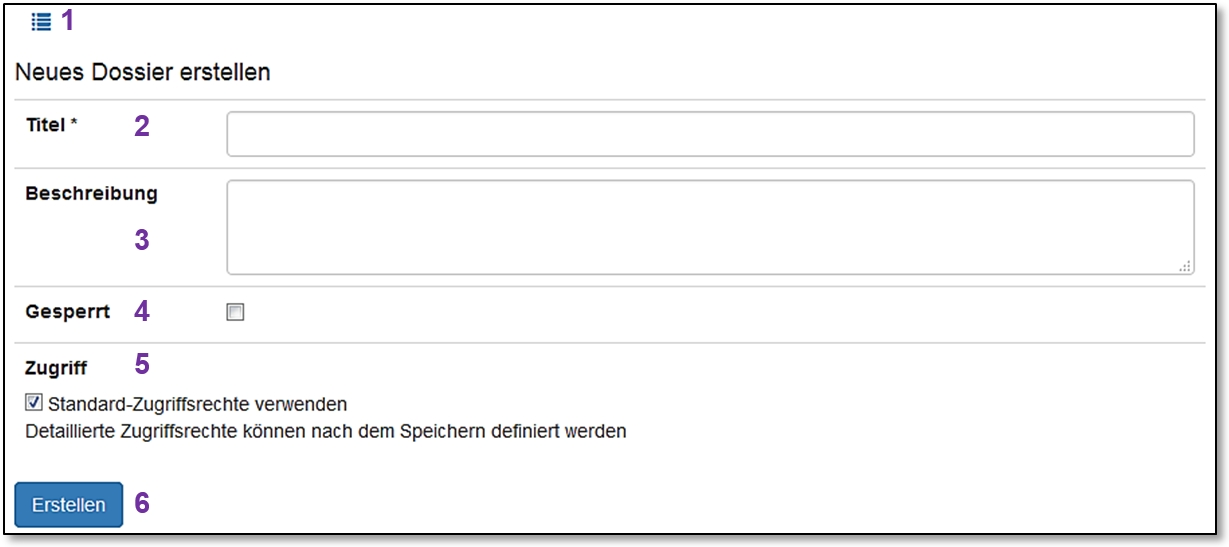
\includegraphics[width=1\linewidth]{../chapters/11_Dokumentenablage/pictures/11-1-1_DossierEingabemaske.jpg}}
\caption{Input form for a new dossier}
% \label{fig:speciation}
\end{figure}

Enter the new dossier's title \col{(2)}. Since more than one dossier can revolve around the same theme, it makes sense to add a date indication in the title, e.g. 'XY Feasibility Study. August 2015'. It is also advisable to first check, before creating a dossier, if a dossier with a similar title already exists. In this case, the exact same text should be used in the title, e.g. 'XY Feasibility Study. August 2015' and 'XY Feasibility Study. December 2015'. If necessary, a detailed description \col{(3)} can be added. Dossiers can be locked against changes. If this function is activated, documents can no longer be added to or removed from the dossier. To do so, check the 'Locked' check-box \col{(4)}. The dossier is now no longer available for selection in the drop-down menu of documents. If needed, dossiers can be protected by access rights. If no special access rights are needed, keep the 'Use default access rights' check-box \col{(5)} checked. If the dossier should only be accessible for certain user groups / users, remove the check-mark. You can later specify which user(s) or which group(s) can view the dossier. For information about access rights, see chapter \ref{bkm:Ref442273510}. \newline

When all desired information is entered, the dossier is created by clicking on the 'Create' button \col{(6)}. To go back to the overview / list of all dossiers, click on the list symbol 
\includegraphics[height=12pt]{/Icons/Listensymbol_zurueck.jpg} \col{(1)}.

\vspace{\baselineskip}

When a dossier is created with the 'Create' button, the following view appears:

\begin{figure}[H]
\center{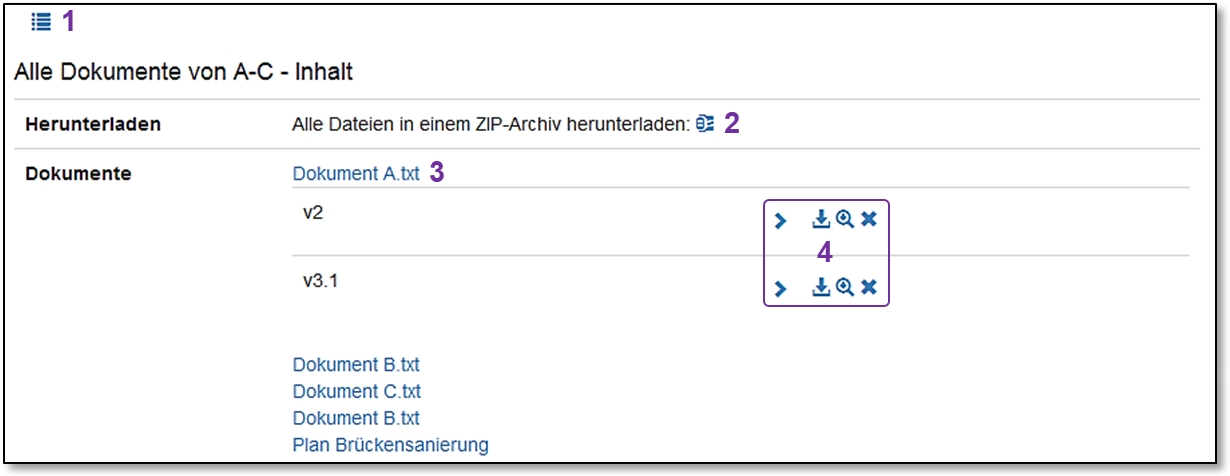
\includegraphics[width=1\linewidth]{../chapters/11_Dokumentenablage/pictures/11-1-1_UebersichtEinesDossiers.jpg}}
\caption{Overview of the dossier}
% \label{fig:speciation}
\end{figure}

The dossier entry is now visible. Click on the ZIP symbol 
\includegraphics[height=12pt]{/Icons/ZIPSymbol.jpg} \col{(2)} to download the documents contained in this dossier. You will also see a list of all the documents contained in this dossier. Click in the blue document title \col{(3)} to open the options (see option explanations below). It is specified which of the major or minor versions of the document is linked to the dossier. Click again on the blue document title to close the options.

Click on the list symbol 
\includegraphics[height=12pt]{/Icons/Listensymbol_zurueck.jpg} \col{(1)} to go back to the overview.

\vspace{\baselineskip}

The assignment of documents to dossiers can be made under the 'Documents' menu item (a subcategory of the 'Document Management' menu item in the menu on the left). To add documents to a dossier, the documents must first be uploaded (see chapter \ref{bkm:Ref442769978}).

\subsubsection{Viewing and editing dossiers}

The following options are available in the dossier overview:

\begin{figure}[H]
\center{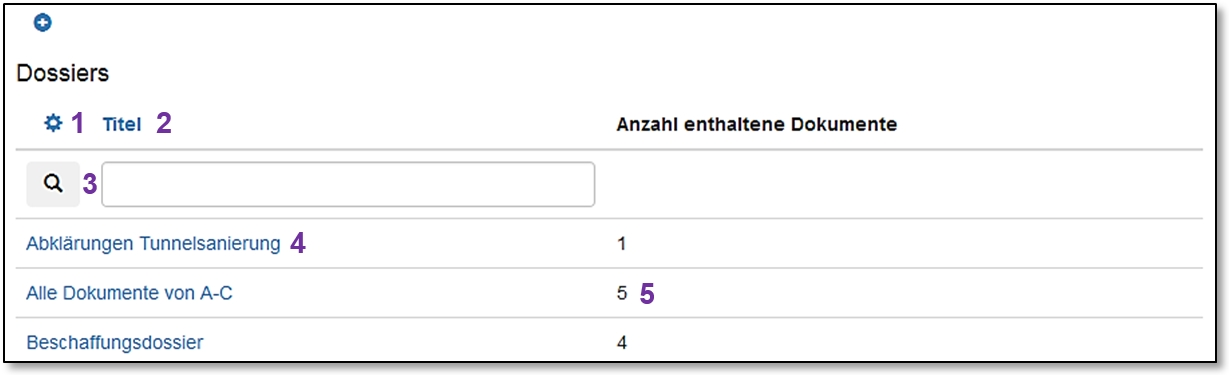
\includegraphics[width=1\linewidth]{../chapters/11_Dokumentenablage/pictures/11-1-2_UebersichtAllerDossiers.jpg}}
\caption{Overview of all dossiers}
% \label{fig:speciation}
\end{figure}

You can hide and show columns with the configuration symbol 
\includegraphics[height=12pt]{/Icons/SpaltenEinst.jpg} \col{(1)} (This can't be changed in the dossier overview since there's only one column). By clicking on 'Title' \col{(2)}, the dossiers are sorted from A to Z. With another click, they are sorted from Z to A.

\vspace{\baselineskip}

\textbf{Search:} You can search for dossiers in the overview. Without using a placeholder (*), you can directly enter a keyword and click on the magnifying glass symbol 
\includegraphics[height=12pt]{/Icons/Lupe_kl.jpg} \col{(3)} or hit 'Enter'. All dossiers containing the keyword will be listed. \newline

By clicking on the dossier title \col{(4)} you switch directly to the detailed and editing view of the dossier. In the overview you can also see how many documents are linked to a dossier  \col{(5)}. Deleting dossiers is not possible at the moment. \newline

If you open a dossier by clicking on its title \col{(4)}, you can also see next to its title and description all the documents contained in the dossier:

\begin{figure}[H]
\center{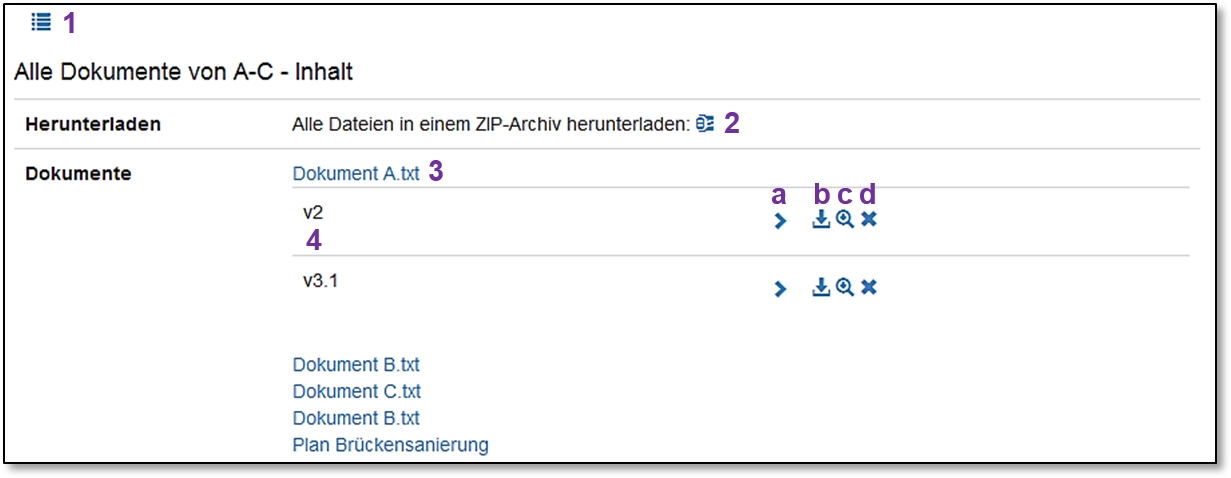
\includegraphics[width=1\linewidth]{../chapters/11_Dokumentenablage/pictures/11-1-2_DetailsEinesDossiers.jpg}}
\caption{Detailed view of a dossier}
% \label{fig:speciation}
\end{figure}

Clicking the list symbol 
\includegraphics[height=12pt]{/Icons/Listensymbol_zurueck.jpg} \col{(1)} returns you to the dossier overview. You can download all documents in a ZIP archive by clicking the ZIP symbol 
\includegraphics[height=12pt]{/Icons/ZIPSymbol.jpg} \col{(2)}. A dialog box appears (depending on the browser you are using) in which you can choose if you want to save the ZIP archive on your computer or just open it. \newline

You will also see the list of all documents contained in the dossier. Click on the blue document title \col{(3)} to display further options. The document version linked to the dossier is specified \col{(4)}. \newline

The following options are available:
The cross 
\includegraphics[height=12pt]{/Icons/Kreuzchen.jpg} \col{(d)} enables you to remove a specific version of a linked document. You need to confirm the security message with 'OK'.

\begin{figure}[H]
\center{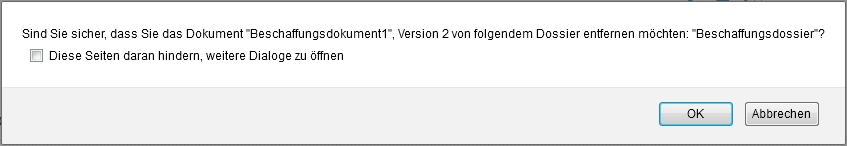
\includegraphics[width=.6\linewidth]{../chapters/11_Dokumentenablage/pictures/11-1-2_DokLoeschen_Meldung.jpg}}
% \caption{Detailansicht des Dossiers}
% \label{fig:speciation}
\end{figure}

The magnifying glass symbol 
\includegraphics[height=12pt]{/Icons/Lupe.jpg} \col{(c)} directs you to the document entry. You can change the document entry, upload a new document version, etc. For details on document management, see chapter \ref{bkm:Ref442273482}. The download symbol 
\includegraphics[height=12pt]{/Icons/Download.jpg} \col{(b)} enables you to download a specific document version (that is not the entire dossier). Depending on the document type, you have the possibility to preview a specific document online. If this option is available, a right-pointing arrow 
\includegraphics[height=12pt]{/Icons/Pfeil_rechts.jpg} \col{(a)} is displayed. Clicking on the arrow opens the preview in a small window. Clicking again on the now downwards-pointing arrow closes the preview.

\begin{figure}[H]
\center{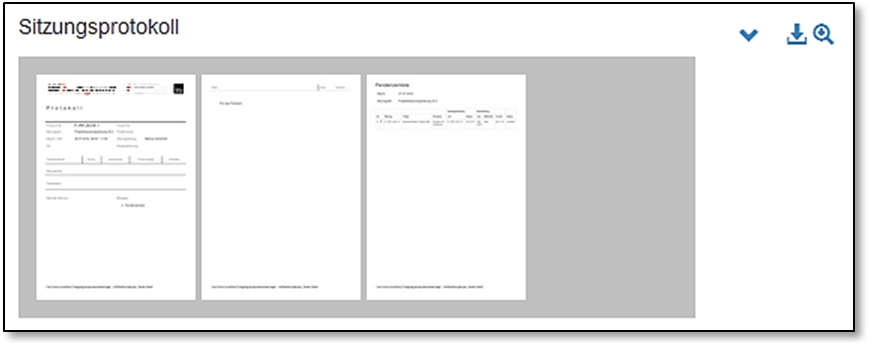
\includegraphics[width=0.75\linewidth]{../chapters/11_Dokumentenablage/pictures/11-1-2_Vorschau.jpg}}
\caption{A document preview}
% \label{fig:speciation}
\end{figure}

\pagebreak

Clicking on one of the previewed pages opens a detailed preview of the page:

\vspace{\baselineskip}

\begin{wrapfigure}[12]{r}{9cm}   % [x] Wie manche Zeile soll sich um die Grafik "brechen"
  \vspace{-30pt}      % Grundwert war 20; mit 30 schön oben beim Text ausgerichtet
  \begin{center}
    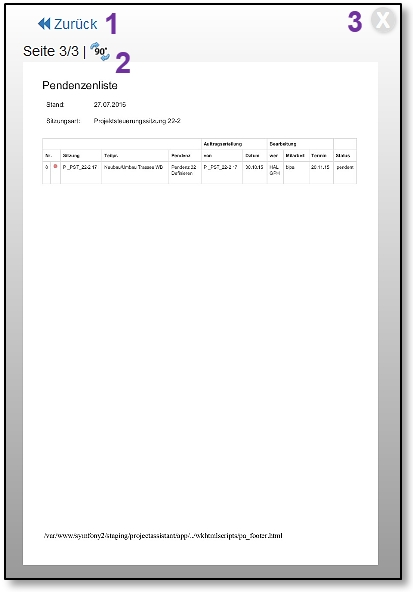
\includegraphics[height=110mm]{../chapters/11_Dokumentenablage/pictures/11-1-2_VorschauDetails.jpg}
  \end{center}
  \vspace{-20pt}
  \caption{A detailed document preview}
  \vspace{-10pt}
\end{wrapfigure}
At the top left, the document navigation shows how many pages the document contains and enables you to browse through the document pages with the 'Previous' and 'Next' buttons \col{(1)}. If needed (for example for a map or a plan) you can use the '90°'-Symbol to rotate a page - another click rotates the page a further 90°, etc. The preview can be closed with the 'X' button \col{(3)}.

\vspace{5cm}

\subsubsection{Dossier access rights}
\label{bkm:Ref442273510}
For every dossier, you can specify who can read, edit, and/or delete it (deleting dossiers is not possible at the moment). You can assign access rights to one or more group(s) or user(s). The procedure is described in chapter \ref{bkm:Ref442869495} and is similar to setting access rights for documents.

\pagebreak
\subsection{Documents}
\label{bkm:Ref442273482}

\subsubsection{Document overview (Searching for documents)}
\label{bkm:Ref443047823}

In the menu on the left, select the menu item 'Document Management' and the subcategory 'Documents'. In the overview, the entered / uploaded documents are listed.

\begin{figure}[H]
\center{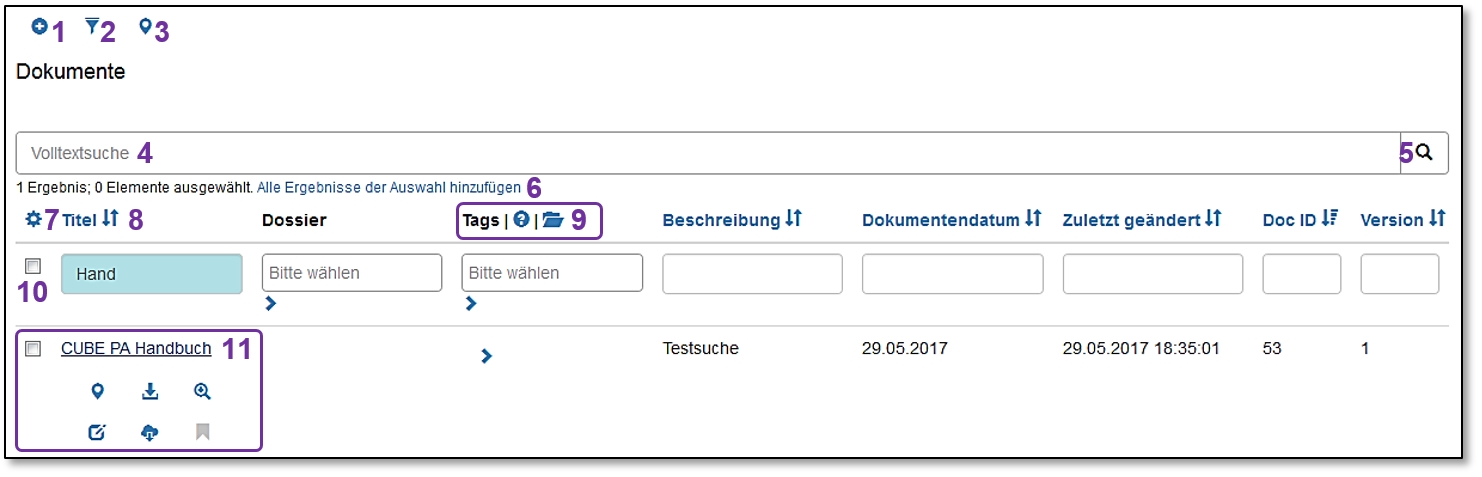
\includegraphics[width=1\linewidth]{../chapters/11_Dokumentenablage/pictures/11-2-1_DokumentenUebersicht.jpg}}
\caption{Overview of the entered documents}
% \label{fig:speciation}
\end{figure}

To upload new documents, click on the plus symbol 
\includegraphics[height=12pt]{/Icons/Plussymbol.jpg} \col{(1)}. More information is provided in chapter \ref{bkm:Ref442770648}. The filter symbol 
\includegraphics[height=12pt]{/Icons/Filter.jpg} \col{(2)} allows you to show or hide the advanced filter functions (see below 'Advanced filter' (\ref{bkm:Ref201704051})). The pin symbol 
\includegraphics[height=12pt]{/Icons/Nadelsymbol.jpg} (toggle map) \col{(3)} allows you to show or hide Google Maps. On the map, all documents related to the search query and linked to Google Maps are shown. The full text search \col{(4)} searches the entries according to keywords. After entering the keyword, click on the magnifying glass symbol 
\includegraphics[height=12pt]{/Icons/Lupe_kl.jpg} \col{(5)} or hit 'Enter'. More than one keyword can be used. If you are searching for a particular word group, enter the word between quotation marks. With the full text search, the titles of documents and dossiers, the tags, and if technically possible, the document contents are searched. Under the full text search, you can see how many data entries were found \col{(6)}.\\
The configuration symbol 
\includegraphics[height=12pt]{/Icons/SpaltenEinst.jpg} \col{(7)} enables you to hide unused columns. After selecting the desired columns click 'Apply' and the view will be updated.\newline
  \newline
In addition to the full text search, you can search in the blue headings \col{(8)}, or use the drop-down menus to choose which documents should be displayed. Clicking on the blue headings sorts the entries from A to Z by this column content. Clicking again sorts them from Z to A. \newline
Uploaded documents can be labeled with tags \col{(9)}. More information about tags is provided in chapter \ref{bkm:Ref442275849}. \\
The check boxes 
\includegraphics[height=12pt]{/Icons/selectbox.jpg} \col{(10)} allow you to select documents (one or many) to apply actions like 'Download', 'Send as Email attachment', and 'Send in print format' to the selection. For further information, see chapter \ref{bkm:Ref201705445} (Document cart).

Clicking on a listed data entry \col{(11)} (in the title column, blue text), shows further options. Another click hides the options. The options are explained below.

\vspace{\baselineskip}

\textbf{Advanced filter:}\\
\label{bkm:Ref201704051}

The filter symbol 
\includegraphics[height=12pt]{/Icons/Filter.jpg} \col{(1)} allows you to show or hide the advanced filter functions:

\begin{figure}[H]
\center{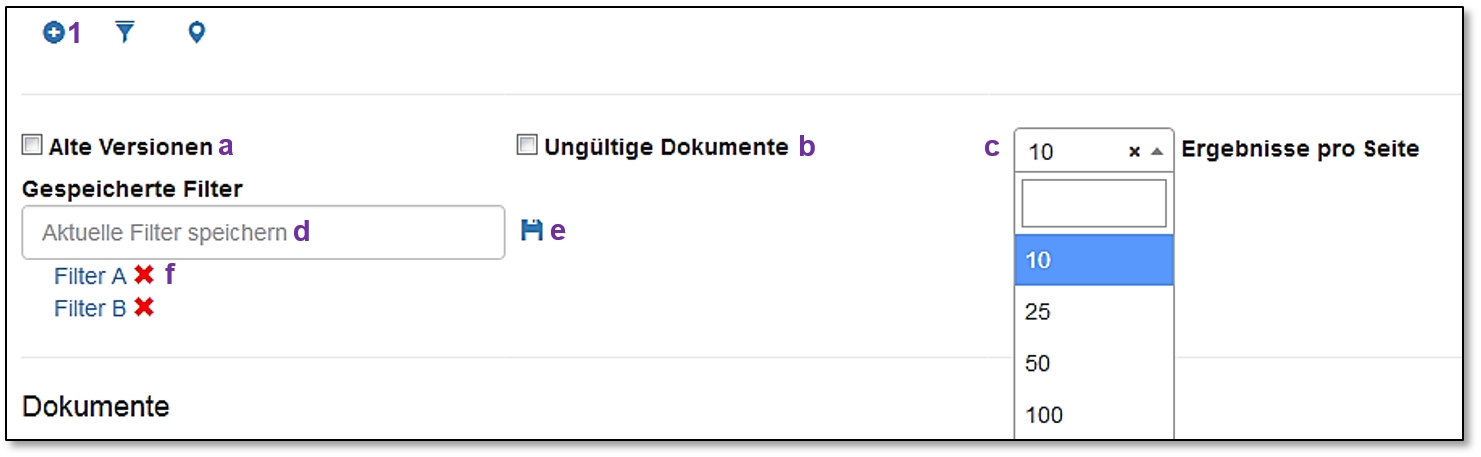
\includegraphics[width=.8\linewidth]{../chapters/11_Dokumentenablage/pictures/11-2-1_FilterEinstellen.jpg}}
\caption{Saving filter settings}
% \label{fig:speciation}
\end{figure}

To include old versions and/or revoked documents in the search, check the 'Show old versions' \col{(a)} and/or 'Show revoked documents' \col{(b)} check-boxes. Under 'Results per page' \col{(c)}, you can select the number of data entries to be displayed on a page.\\
You can save filter setting for future use. This takes into account the full text search, title entries, document IDs, and further columns. The number of results per page is not saved in the filter settings.\\
Once you've entered the desired filter settings, enter a title for the filter \col{(d)} then click on the save symbol 
\includegraphics[height=12pt]{/Icons/Diskette.jpg} \col{(e)}. All saved filter settings are displayed \col{(f)}. A saved filter setting can be removed by clicking on the red cross 
\includegraphics[height=12pt]{/Icons/roKreuzchen.jpg} \col{(f)}.


\subsubsection{Uploading documents}
\label{bkm:Ref442863508}\label{bkm:Ref442787515}\label{bkm:Ref442778397}\label{bkm:Ref442770648}\label{bkm:Ref442769978}

\begin{figure}[H]
\center{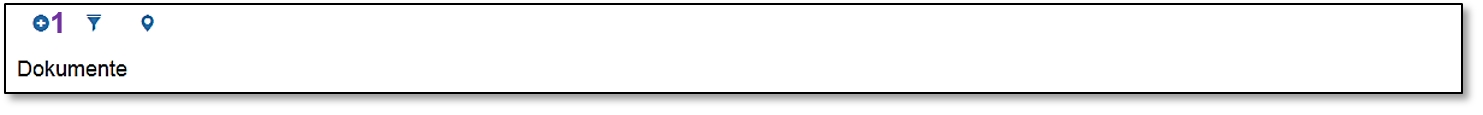
\includegraphics[width=1\linewidth]{../chapters/11_Dokumentenablage/pictures/11-2-2_DokumenteHochladen.jpg}}
% \caption{Neues Dokument hochladen}
% \label{fig:speciation}
\end{figure}

Click on the plus symbol 
\includegraphics[height=12pt]{/Icons/Plussymbol.jpg} \col{(1)}. The input form for a new document appears:

\begin{figure}[H]
\center{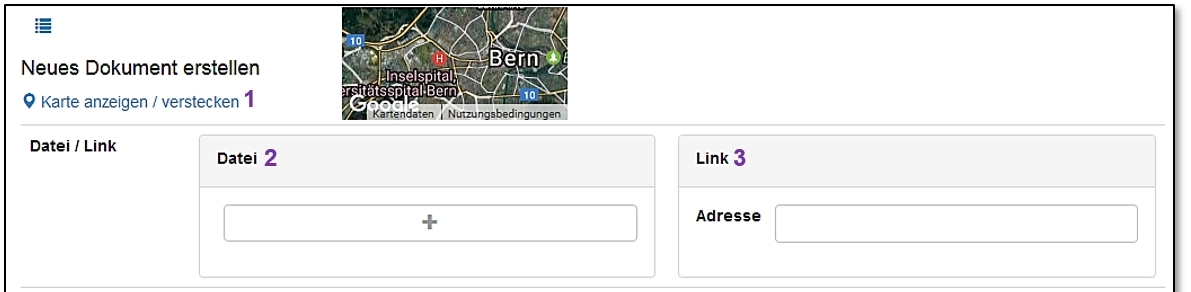
\includegraphics[width=1\linewidth]{../chapters/11_Dokumentenablage/pictures/11-2-2_NeuesDokuErstellen_A.jpg}}
\caption{Input form for a new document}
% \label{fig:speciation}
\end{figure}

Click on the 'Toggle map' link \col{(1)} to show Google Maps, or to switch from a small view to a larger one. More information about linking a document to Google Maps can be found in chapter \ref{bkm:Ref442545553}. \newline

You can now choose whether you want to upload a file \col{(2)} or save an Internet link \col{(3)}.

\vspace{\baselineskip}

\textbf{Uploading a file:} \col{(2)}
\begin{figure}[H]
\center{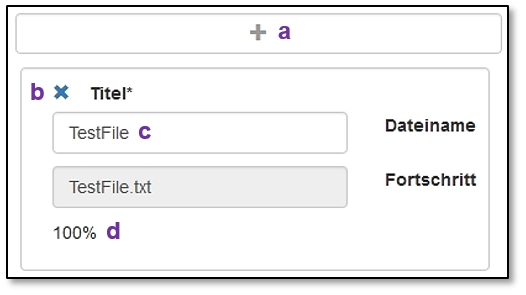
\includegraphics[width=.5\linewidth]{../chapters/11_Dokumentenablage/pictures/11-2-2_Dateititel.jpg}}
\caption{Uploading a new document}
\end{figure}

Click on the gray plus symbol 
\includegraphics[height=12pt]{/Icons/plus_grau.jpg} \col{(a)} and select the desired file or files. Alternatively, you can drag and drop the desired file or files over the 'plus area'. Once a file has been selected / dropped in the 'plus area', additional fields \col{(b-d)} appear. If you're uploading a big file, you can see the upload progress of the file \col{(d)} and see if the file was completely uploaded. The title field is a mandatory field. It is copied from the file name field \col{(c)} but can be changed at any time. If you've uploaded the wrong file, click on the small cross 
\includegraphics[height=12pt]{/Icons/Kreuzchen.jpg} \col{(b)} to remove the file / entry. \\
You can add additional files. To do so, repeat the above steps. 

\vspace{\baselineskip}

\textbf{Saving an link:} \col{(3)}
\begin{figure}[H]
\center{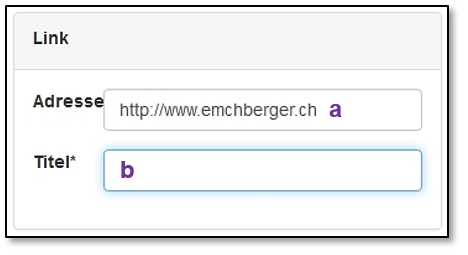
\includegraphics[width=.5\linewidth]{../chapters/11_Dokumentenablage/pictures/11-2-2_Linktitel.jpg}}
\caption{Saving a link}
\end{figure}

Under 'Address' \col{(a)}, enter the desired url. An additional 'Title' field \col{(b)} appears (mandatory field), in which you'll need to enter a title for the link.\\

If you've entered an invalid url, the following error message appears:

\begin{figure}[H]
\center{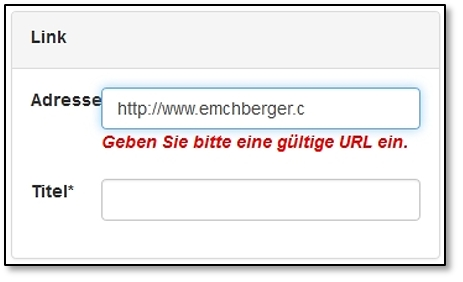
\includegraphics[width=.5\linewidth]{../chapters/11_Dokumentenablage/pictures/11-2-2_Link_Fehler.jpg}}
\caption{Saving a link}
\end{figure}

\vspace{\baselineskip}

If you've uploaded a file or entered a url, you can fill out the following fields:

\begin{figure}[H]
\center{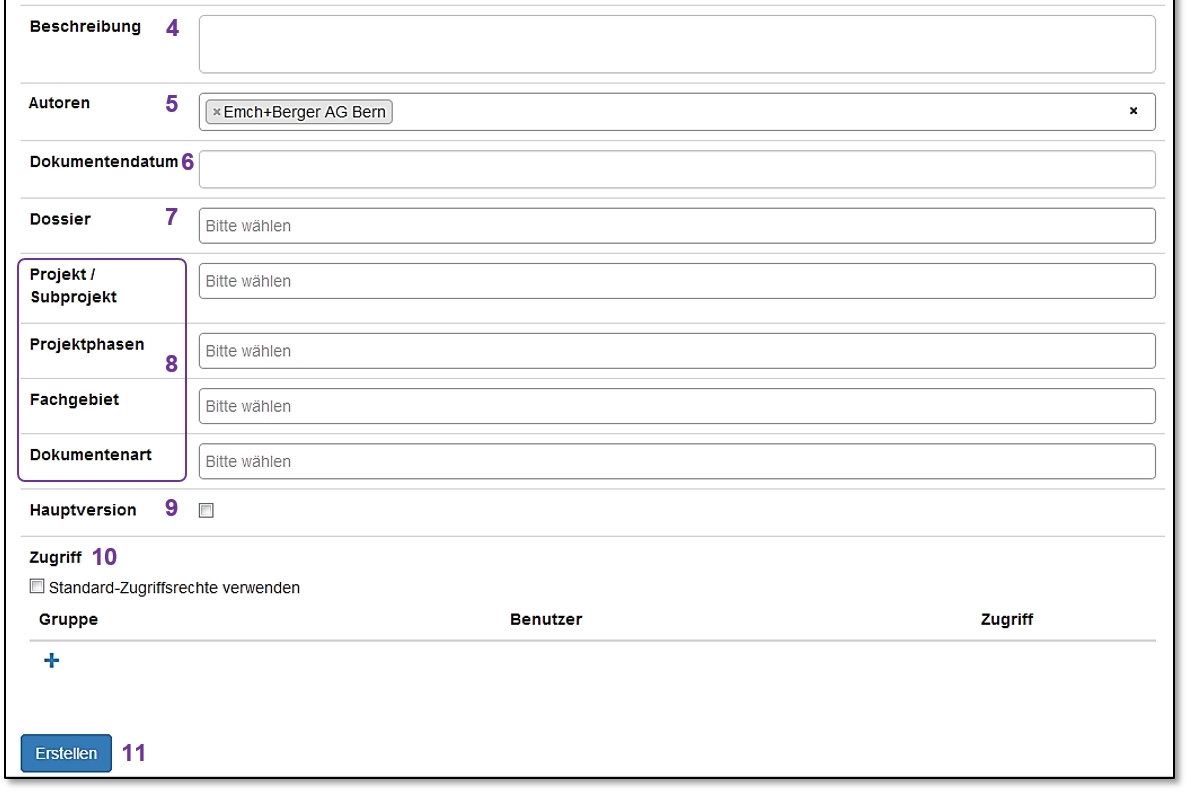
\includegraphics[width=1\linewidth]{../chapters/11_Dokumentenablage/pictures/11-2-2_NeuesDokuErstellen_B.jpg}}
\caption{Input form for a new document}
% \label{fig:speciation}
\end{figure}

\vspace{\baselineskip}

In the description \col{(4)}, you can enter additional notes. Under authors \col{(5)}, you can use a drop-down menu to select the authors. An author must already exist. If an author is not on the list, they can be added by the administrator. You have the option to enter a document date \col{(6)}. To assign a document to a dossier (see chapter \ref{bkm:Ref442544219}), select the dossier from the drop-down menu \col{(7)} (the dossier must already exist). A document can be assigned to more than one dossier. Click again on the drop-down menu to select more dossiers for the document. 'Tags' \col{(8)} can be defined and then assigned to a document. It is then possible to search for specific tags to find documents of specific projects, project phases, areas of expertise, or document types. Tag themes (e.g. area of expertise) as well as individual tags (e.g. level crossings, lighting, operation, etc.) can only be defined or added by the administrator. If a tag is missing, please contact the administrator. \newline

In case of a multiple file upload, a separate entry, but with the same information (description, authors, dossier, etc.) is created for each uploaded document. This is a time-saving procedure, especially for the compilation of a dossier with many documents having the same description, authors, etc. \newline

%If a document is no longer valid, it can be excluded from search results by checking the 'Revoked' check-box \col{(8)}. This function is not to be confused with the versioning of documents, whereby old versions of a document are not displayed in search results by default. \newline

You can define whether a newly uploaded file is a major version (V2, V3, etc.) or a minor version (V3.1, V3.2, etc.) of a document. If the new document is a major version check the 'Major version' check-box \col{(9)}. You can assign standard access rights to a document \col{(10)} or only authorize its access to specific persons. Access rights can be adapted and expanded any time later in the edit mode. Refer to chapter \ref{bkm:Ref442869495} for more information about access rights. In order to create a document, at least one person must have access rights to the documents (usually the person creating the document).

Once all necessary information is entered, the document is uploaded with the 'Create' button \col{(11)} and the entries are saved. \newline

\textbf{Note:} A document can only be replaced by one other document. When attempting to drag several documents into the upload window, the following error message appears:

\begin{figure}[H]
\center{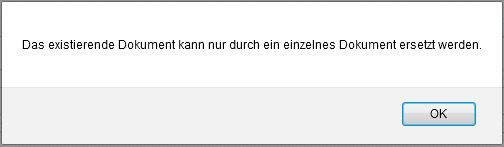
\includegraphics[width=0.75\linewidth]{1122_FehlerDokumentErsetzen.jpg}}
\caption{Error message for uploading more than one file}
% \label{fig:speciation}
\end{figure}

\textbf{Note:} If only the metadata of a document is modified and saved, no new document version will be created. The changes in the metadata will however appear in the document change log. Similarly, if the same file is uploaded (in which no changes were made) or if a document was checked-out then checked-in without any changes being made, CUBE PA does not create a new document version. The following message appears:

\begin{figure}[H]
\center{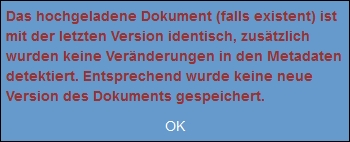
\includegraphics[width=0.5\linewidth]{../chapters/11_Dokumentenablage/pictures/11-2-2_Meldung_gleicheDatei.jpg}}
\caption{Message: No new document version created}
% \label{fig:speciation}
\end{figure}

In order to continue working, you must first click 'OK' in the above dialog.

\subsubsection{Linking document with Google Maps}
\label{bkm:Ref442545553}
Documents can be linked to Google Maps. This way documents related to a specific location can be found, edited or downloaded. \\
Switch to the edit mode of the desired document with the editing symbol 
\includegraphics[height=12pt]{/Icons/Bearbeiten.jpg} (in the view mode, you can only view Google Maps links but you can't create, add or remove a link).

% \vspace{\baselineskip}
\vspace{2mm}

\begin{wrapfigure}[15]{l}{6.5cm}
\vspace{-15pt}
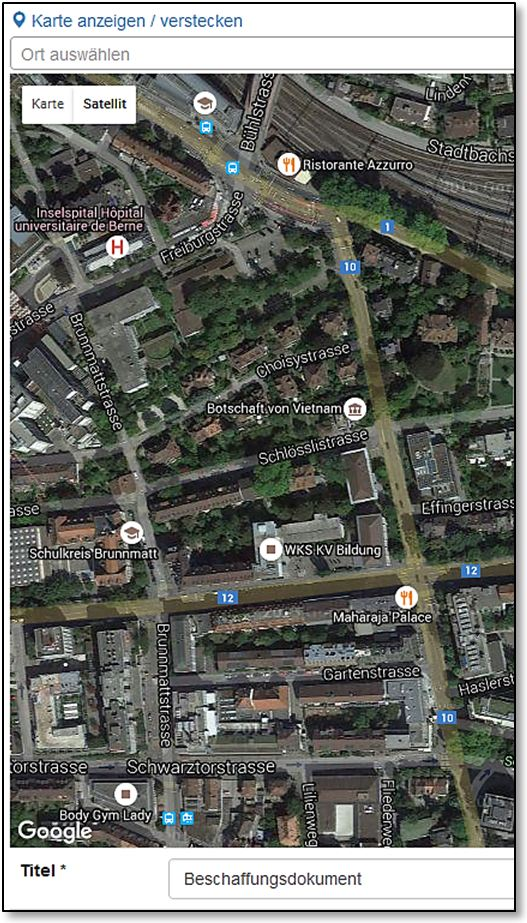
\includegraphics[height=110mm]{1123_GoogleMap.jpg}
% \caption{Status ändern}
\end{wrapfigure}

To link a document to a location on the map, double click on the object / desired location on the map. You can also select a predefined location. To do so, click on the 'Select location' input field above the map and select the desired location.

\vspace{4mm}

\hspace{15mm} 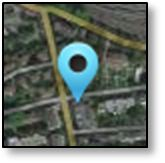
\includegraphics[height=20mm]{1123_GoogleMapNadel.jpg}

The above pin appears. You can later move this pin to another location by drag \& drop. 

\hspace{15mm} 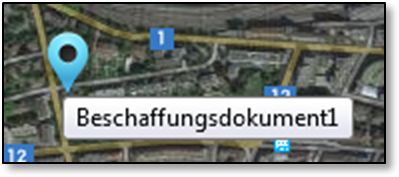
\includegraphics[height=20mm]{1123_GoogleMapText.jpg}

Hover the mouse over the pin to see which documents are linked to its location. \\

Repeat the above steps to add more Google Maps links. If you want to remove a specific link, right-click on it. The following dialog appears, and you need to confirm it by clicking 'OK':

\begin{figure}[H]
\center{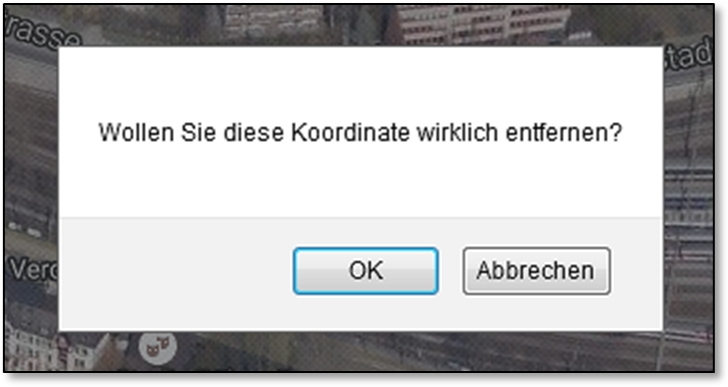
\includegraphics[width=0.5\linewidth]{../chapters/11_Dokumentenablage/pictures/11-2-3_DialogLoeschen.jpg}}
\caption{Removing a link}
% \label{fig:speciation}
\end{figure}

\vspace{\baselineskip}
\pagebreak

\textbf{Handling with Google Maps in CUBE PA}:

The handling with Google Maps in CUBE PA is like the handling of Google Maps in an Internet browser. Click and hold the left mouse button to pan the map. If your mouse has a scroll wheel, you can use it to zoom in and out of the map. (Function keys such as Shift, Ctrl and Alt do not function in map handling).

\vspace{\baselineskip}

\textbf{Searching for a location:} 

\begin{figure}[H]
\center{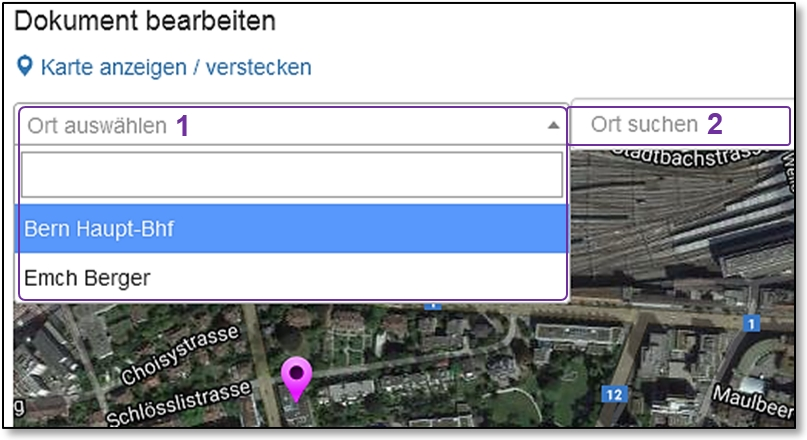
\includegraphics[width=0.6\linewidth]{../chapters/11_Dokumentenablage/pictures/11-2-3_GeographischSuchen.jpg}}
\caption{Searching for a location}
% \label{fig:speciation}
\end{figure}

When Google Maps is displayed in the document overview (click on 'Toggle map'), all documents with a Google Maps link are shown. You can now select a location from the drop-down menu \col{(1)} or search for a location \col{(2)} by typing the information in the field and hitting 'Enter'. Google Maps will navigate to the desired location and display all documents that are linked to it. If you have filtered the document list in the document overview, only the filtered documents will appear on the map. \newline

\pagebreak
\textbf{Filtering documents by geographic area:} \\

\begin{wrapfigure}[9]{r}{7cm}
  \vspace{-35pt}
  \begin{center}
    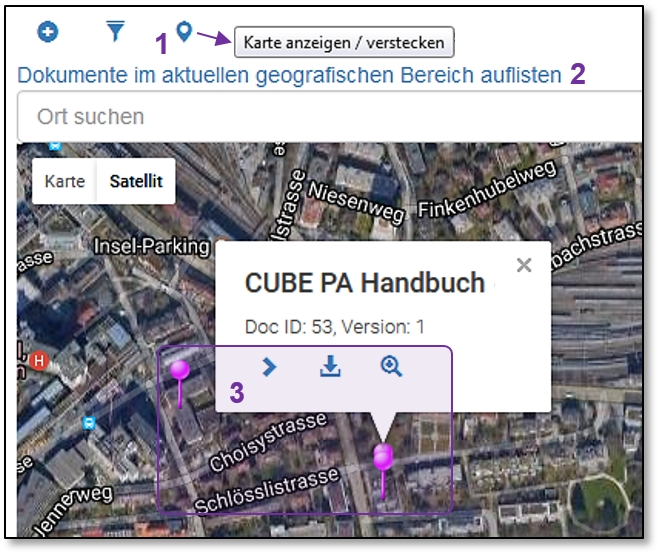
\includegraphics[height=55mm]{../chapters/11_Dokumentenablage/pictures/11-2-3_GeoBereichFilter.jpg}
  \end{center}
  \vspace{-20pt}
  % \caption{Geografische Bereiche filtern}
  \vspace{-10pt}
\end{wrapfigure}
You have option to filter documents that are in the same geographic area or that have the same or close coordinates. To do so, click on 'Toggle map' \col{(1)} to show Google Maps. The function 'List documents in currently visible area' \col{(2)} now appears. Click on it to set a geographic filter:

\vspace{1cm} 

\begin{wrapfigure}[12]{r}{8cm}
  \vspace{-25pt} 
  \begin{center}
    \includegraphics[height=70mm]{../chapters/11_Dokumentenablage/pictures/11-2-3_GeoBereichResult.jpg}
  \end{center}
  \vspace{-20pt}
  % \caption{Dokumenten in einem gemeinsamen geografischen Bereich}
  \vspace{-10pt}
\end{wrapfigure}
'Geographic filter set' appears above the search / filter fields. Only documents with close geographic coordinates are displayed. In this example, two documents are listed. These were the two documents indicated with pins on the map in the previous screen shot \col{(3)}. These are the two documents of the search result. To remove the geographic filter, click on the small cross next to 'Geographic filter set' \col{(4)}. Then click on the magnifying glass symbol \includegraphics[height=12pt]{/Icons/Lupe.jpg} to display the unfiltered list.

\subsubsection{Working with the uploaded documents}
\label{bkm:Ref442801819}

\begin{figure}[H]
\center{\includegraphics[width=1\linewidth]{../chapters/11_Dokumentenablage/pictures/11-2-4_FunktionenHochgDateien.jpg}}
\caption{Options for uploaded documents}
% \label{fig:speciation}
\end{figure}

You can search for documents in the document overview (see chapter \ref{bkm:Ref443047823}). Click on the title of the desired document (blue font) \col{(1)} to see the various document options. The options are displayed. Click again on the document title to hide the options. \newline

If the document is linked to Google maps, click on the pin symbol \includegraphics[height=12pt]{/Icons/Nadelsymbol.jpg} \col{(2)} to go directly to the document location in the map. The pin symbol is only displayed if a link to Google Maps exists (see chapter \ref{bkm:Ref442545553}). The following window is opened:

\begin{figure}[H]
\center{\includegraphics[width=0.5\linewidth]{../chapters/11_Dokumentenablage/pictures/11-2-4_DokAufGoogleMaps.jpg}}
% \caption{Das Menü in CUBE PA}
% \label{fig:speciation}
\end{figure}

From this window, you have the option to open the document preview, to download the document, or to display the document entry. Click on the cross in the upper right corner of the dialog box to close the window. \newline

Click on the arrow symbol \includegraphics[height=12pt]{/Icons/Pfeil_rechts.jpg} \col{(3)} to preview the document in the document overview - insofar as the preview of the uploaded file format is supported. Click again on the arrow symbol \includegraphics[height=12pt]{/Icons/Pfeil_unten.jpg} to close the preview. More information about the preview is given later. \newline

You can also download the document directly \includegraphics[height=12pt]{/Icons/download.jpg} \col{(4)}, view the document entry \includegraphics[height=12pt]{/Icons/Lupe.jpg} \col{(5)} or edit the document entry \includegraphics[height=12pt]{/Icons/Bearbeiten.jpg} \col{(6)}. \newline

To edit a document online, it must be checked out with the symbol \includegraphics[height=12pt]{/Icons/Auschecken.jpg} \col{(7)}. The procedure is described in detail in chapter \ref{bkm:Ref442776572}. Click the gray favorite symbol \includegraphics[height=12pt]{/Icons/DokuFlag_grau.jpg} \col{(8)} to add a document to your personal favorites. The symbol will turn red and the document will appear in your personal overview (see chapter \ref{bkm:Ref132000001}). Click again on the favorite symbol \includegraphics[height=12pt]{/Icons/DokuFlag_rot.jpg} to remove the document from your favorites. \newline

\pagebreak
\subsubsection{Document view}
\label{bkm:Ref443047930}

\begin{wrapfigure}[18]{l}{9.5cm}
\vspace{-15pt}
\includegraphics[height=105mm]{../chapters/11_Dokumentenablage/pictures/11-2-5_Dokumentenansicht.jpg}
% \caption{Status ändern}
\end{wrapfigure}

If you click on the magnifying glass symbol \includegraphics[height=12pt]{/Icons/Lupe.jpg} the document entry is opened in view mode. Next to the title \col{(1)}, all information (e.g. author(s), tags that were added when uploading or when editing the document (see chapter \ref{bkm:Ref442778397})). When information is missing, the corresponding fields are either empty or not displayed. The document version, the timestamp and the editor \col{(2)} are displayed below the title. \newline

To download the document, click the download symbol \includegraphics[height=12pt]{/Icons/Download.jpg} or the file name \col{(3)} in the 'File' field. The usual download window of your browser will open, and you can choose whether to open or save the document. Click on the send icon \includegraphics[height=12pt]{/Icons/Versandsymbol.jpg} \col{(4)} to send this document by Email to a person of your choice (see chapter \ref{bkm:Ref201701127} for more information). Click on the document cart icon \includegraphics[height=12pt]{/Icons/shoppingcart_g.jpg} \col{(5)} to add the document to the cart. The icon color changes to red when the document is in the cart: \includegraphics[height=12pt]{/Icons/shoppingcart_r.jpg}. Click again on the icon to remove the document from the cart. The document cart is described in chapter \ref{bkm:Ref201705445}. \newline

Click on the favourites icon \includegraphics[height=12pt]{/Icons/DokuFlag_grau.jpg} \col{(6)} to be able to see the document in your personal overview. The icon color changes to red when the document is added to your favourites: \includegraphics[height=12pt]{/Icons/DokuFlag_rot.jpg}. Click on the red icon to remove the document from your personal overview. \newline

'Static Link to Latest File-Version' \col{(7)} refers to the latest version of the document. You can send this link per e-mail for example, ensuring that the receiver will always be directed to the latest document version.

The first pages of the document are displayed in reduced view under 'Preview' \col{(8)}.

\vspace{\baselineskip}

Click on one of the previewed pages \col{(9)} to open the selected page in preview mode. Click on the gray cross \includegraphics[height=12pt]{/Icons/X_Button.jpg} \col{(a)} in the top right corner of the preview to close it. Click \includegraphics[height=11pt]{/Icons/Weiter.jpg} and \includegraphics[height=11pt]{/Icons/Zurueck.jpg} \col{(b)} to browse through the document pages. The number of pages \col{(c)} is displayed under the page navigation buttons. You can rotate the pages 90° with the 90° symbol \includegraphics[height=12pt]{/Icons/90Grad.jpg} \col{(d)}.

\begin{figure}[H]
\center{\includegraphics[width=1\linewidth]{../chapters/11_Dokumentenablage/pictures/11-2-5_Dokumentenvorschau.jpg}}
\caption{Document preview}
% \label{fig:speciation}
\end{figure}

\textbf{Additional options in the document view:}

\begin{figure}[H]
\center{\includegraphics[width=1\linewidth]{../chapters/11_Dokumentenablage/pictures/11-2-5_Dokumentenoptionen.jpg}}
\caption{Additional options for uploaded documents}
% \label{fig:speciation}
\end{figure}

In the 'Checkout file' field \includegraphics[height=12pt]{/Icons/Auschecken.jpg} \col{(1)}, the latest document version can be checked-out (see chapter \ref{bkm:Ref442780171}). If the document is assigned to a dossier, clicking on the dossier title \col{(2)} leads you to the corresponding dossier. A document can be assigned to multiple dossiers. \newline 

\vspace{\baselineskip}

Under 'Changelog', click on the arrow symbol \includegraphics[height=12pt]{/Icons/Pfeil_rechts.jpg} \col{(3)} to view the changes made to the document.

\begin{figure}[H]
\center{\includegraphics[width=1\linewidth]{1125_Aenderungshistorie.jpg}}
\caption{Viewing document changelog}
% \label{fig:speciation}
\end{figure}

A list with the changes is displayed. The changes made to the document information (e.g. author, tags) and the changes made to the document itself (new versions) are included in the list. Click the download symbol \includegraphics[height=12pt]{/Icons/Download.jpg} \col{(6)} to download an old version of the document or the magnifying glass symbol \includegraphics[height=12pt]{/Icons/Lupe.jpg} \col{(5)} to view an old version of the document. \newline

\begin{wrapfigure}[7]{r}{6cm}
\vspace{-15pt}
\includegraphics[height=40mm]{1125_DokumentAeltereVersion.jpg}
% \caption{Status ändern}
\end{wrapfigure}
If you open an old version of a document, the warning \textcolor{red}{'This is not the latest version of this document!'} appears in the document view. If you download the document in the 'File' field, you will not access the latest document version, but the selected and displayed older document version.

\begin{wrapfigure}[7]{r}{6cm}
% \vspace{-15pt}
\includegraphics[height=35mm]{1125_DokumentBearbeiten.jpg}
% \caption{Status ändern}
\end{wrapfigure}
To edit document information or to upload a new document version, click in the top left of the window on the edit symbol \includegraphics[height=12pt]{/Icons/Bearbeiten.jpg} \col{(1)}. The list symbol \includegraphics[height=12pt]{/Icons/Listensymbol_zurueck.jpg} \col{(2)} takes you back to the document overview. (In the view of an older document version, the edit symbol is hidden. You can only click on the list symbol \includegraphics[height=12pt]{/Icons/Listensymbol_zurueck.jpg} to return to the document overview.)

\vspace{\baselineskip}

\textbf{Details about the changelog} \\
All changes are recorded in the changelog. On the one hand, the changelog records when a new document (a revised version) is uploaded. On the other hand, the changes to the metadata are also recorded in the changelog, without generating a new document version (see chapter \ref{bkm:Ref442863508}).

\begin{figure}[H]
\center{\includegraphics[width=1\linewidth]{../chapters/11_Dokumentenablage/pictures/11-2-5_AenderungshistorieUebersicht.jpg}}
\caption{The changelog in the overview}
% \label{fig:speciation}
\end{figure}

\col{(1)} In the changelog, the document version currently opened in view mode is displayed with a 'bold' font. You also see which version it is. The different entries are separated by a line \col{(2)}. All changes are recorded. First entry: A new file was uploaded and a description (metadata) was added. Second entry: The document was only added to the procurement dossier. You can see when and by whom the changes were made. To open the preview of the current or earlier version of the document, click on the arrow symbol \includegraphics[height=12pt]{/Icons/Pfeil_rechts.jpg} \col{(3)}. Click on one of the preview pages to display it in large format. You have the possibility to browse through the document or to rotate a page 90°. Click on the cross \includegraphics[height=12pt]{/Icons/X_Button.jpg} at the top right to close the large format preview. Click on the arrow symbol (downward pointing \includegraphics[height=12pt]{/Icons/Pfeil_unten.jpg}) to close the small preview.

In the changelog, you can download the current or earlier version of a document using the download symbol \includegraphics[height=12pt]{/Icons/download.jpg} \col{(4)}. Use the magnifying glass symbol \includegraphics[height=12pt]{/Icons/Lupe.jpg} \col{(5)} to get an overview of the corresponding (earlier) document version. You also have the options to change the metadata of an earlier version. To do so, click on the editing symbol \includegraphics[height=12pt]{/Icons/Bearbeiten.jpg} \col{(6)}. Before editing, make sure you have opened the correct document version.

\vspace{\baselineskip}

\textbf{Note:} Changing earlier document versions (metadata, access rights) is only possible via the changelog as described above.

%% bishierher

\pagebreak

\textbf{Uploading a new version of a document}

\vspace{\baselineskip}

\begin{wrapfigure}[13]{r}{6cm}
\vspace{-35pt}
\includegraphics[height=100mm]{1125_DokumentBearbeitenFelder.jpg}
% \caption{Status ändern}
\end{wrapfigure}
In the editing mode, you can complete the document information (see chapter \ref{bkm:Ref442787515}). To upload a new version of a document, click under 'File' on 'Search' \col{(1)} and select the desired file. If needed, other entries (metadata) can be adapted.

\vspace{\baselineskip}

When all necessary entries are made, click 'Apply' \includegraphics[height=12pt]{/Icons/B_Uebernehmen.jpg} at the bottom left to upload the document and to save the entries. The old version (document and metadata) remain stored and can be accessed at any time in the 'Changelog' of the document view.

\vspace{\baselineskip}
\vspace{\baselineskip}

\textbf{Note}: If more than one version of a document are assigned to the same dossier, only the latest version will be included in the dossier (this is done automatically). This should be especially taken into account when uploading new versions of documents. If for example a new version of a document is no longer to be assigned to a certain dossier, the dossier entry should be removed when uploading the document (by clicking on the 'x' in the dossier row \col{(2)}). This way the old version of the document will not be 'overwritten' in the dossier.  

\begin{figure}[H]
\center{\includegraphics[width=1\linewidth]{1125_DokEintragLoeschen.jpg}}
\caption{Remove entry}
% \label{fig:speciation}
\end{figure}


\subsubsection{Document cart}
\label{bkm:Ref201705445}
% Neues Kapitel

The document cart's functionality is similar to that of a shopping cart in an online shop. The document cart enables different functions such as downloading documents in a zip file, sending them directly in an email, or sending plans to be plotted. It is therefore possible to add a certain number of documents to the document cart and then use the desired function on all the documents in the cart.

\vspace{\baselineskip}

Proceed as follows:

\begin{figure}[H]
\center{\includegraphics[width=1\linewidth]{../chapters/11_Dokumentenablage/pictures/11-dkorb_Dokumentenkorb_Uebersicht1.jpg}}
\caption{Using the document cart}
% \label{fig:speciation}
\end{figure}

Using the full text search or the filter, or by browsing through the documents, find the document you wish to add to the cart. Select the document by checking the corresponding check-box \col{(1)}. Repeat the procedure until you have selected all the documents you need to work with. The available options appear above of the list \col{(2)}. You also have the option to use these options under the individual document titles \col{(8)}. \\
Clicking on the document cart icon \col{(3)} gives you the following options: you can either empty the selection (remove all selected documents from the cart) \col{(a)} or show the selection (list of all selected documents in the cart) \col{(b)}:
\begin{figure}[H]
\center{\includegraphics[width=.25\linewidth]{../chapters/11_Dokumentenablage/pictures/11-dkorb_Auswahl.jpg}}
% \caption{Weitere Optionen}
% \label{fig:speciation}
\end{figure}

Clicking on the favourites icon \col{(4)} enables you to show all selected documents as favourites in your personal overview. \\
Click on the download symbol \col{(5)} to download all documents in the cart in a zip file. If you want to send the selected documents by email, click on the send symbol \col{(6)}. You will find more information on the subject in chapter \ref{bkm:Ref201701127} (Sending documents by email). You also have the option to send the selected documents in printed form. To do so, click on the printer icon \col{(7)}. You will find more information about this option in chapter \ref{bkm:Ref20170609127} (Plotting orders to plot centers).

\vspace{\baselineskip}

If the cart only contains one document, more options will be available:

\begin{figure}[H]
\center{\includegraphics[width=.8\linewidth]{../chapters/11_Dokumentenablage/pictures/11-dkorb_weitereOptionen.jpg}}
\caption{Additional options}
% \label{fig:speciation}
\end{figure}

In addition to the options described above, you can click on the magnifying glass symbol \col{(1)} to view the details of the selected document, click on the edit symbol \col{(2)} to make changes to the document, click on the pin symbol \col{(3)} to assign the document to a Google Maps location, or check-out the document \col{(4)}. These buttons correspond to the options that appear under the document title.

\vspace{\baselineskip}

\textbf{Note:} If the selection is shown by clicking on the document cart icon, the icon color turns to red. Similarly, by clicking on the favourites icon for the selection, the color of the icon also turns red \col{(1)}:

\begin{figure}[H]
\center{\includegraphics[width=.75\linewidth]{../chapters/11_Dokumentenablage/pictures/11-dkorb_Dokumentenkorb_Uebersicht2.jpg}}
\caption{Display document cart selection / Stop viewing selection}
% \label{fig:speciation}
\end{figure}

\textbf{Note:} Click on the cross \includegraphics[height=12pt]{/Icons/FilterLoeschen_b.jpg} \col{(2)} to stop viewing the selection. 

\vspace{\baselineskip}

\textbf{Option description:}

\subsubsection{Sending documents by email}
\label{bkm:Ref201701127}
% Neues Kapitel

It is possible to send documents as email attachments to persons of your choice directly from the document list. For transparency and traceability, the sending of documents is recorded in the document changelog.

Click on the send symbol \includegraphics[height=12pt]{/Icons/Versandsymbol.jpg} to send all documents in the cart to one or more email addresses. You can always remove documents you do not want to include in the attachments before sending the email.

\begin{figure}[H]
\center{\includegraphics[width=1\linewidth]{../chapters/11_Dokumentenablage/pictures/11-dkorb_Dok_versenden}}
\caption{Sending documents}
% \label{fig:speciation}
\end{figure}

Entering recipients \col{(1)}: In the 'Recipients' field, enter one or more email addresses. Seperate the email addresses with a semicolon or a blank space.
In the 'Message' field \col{(2)} you can enter some information to be sent to the recipient or recipients. All the selected documents which will be sent to the recipient or recipients are shown. You can always remove documents before sending using the cross symbol \includegraphics[height=12pt]{/Icons/blKreuzchen.jpg} \col{(3)}. The total size of the attachments is shown at the bottom of the list \col{(4)}. Once you've filled out all the necessary information, click on 'Send' \col{(5)} to send the documents.

\vspace{\baselineskip}

A confirmation message appears showing the recipients of the email with the documents:

\begin{figure}[H]
\center{\includegraphics[width=.4\linewidth]{../chapters/11_Dokumentenablage/pictures/11-dkorb_Sendebestaetigung}}
\caption{Sending confirmation}
% \label{fig:speciation}
\end{figure}

You will also receive an email stating which documents were sent to which recipients. If an email could not reach a recipient, this is also stated.

\vspace{\baselineskip}

\subsubsection{Download documents as a zip file}
% Neues Kapitel

You have the option to download all documents in the document cart as a zip archive. To do so, click on the download symbol in the document cart options.

\vspace{\baselineskip}

The download window of your browser appears. Choose whether you want to open the zip file in the windows explorer or save it on your computer:

\begin{figure}[H]
\center{\includegraphics[width=.5\linewidth]{../chapters/11_Dokumentenablage/pictures/11-dkorb_DokDownload}}
\caption{Download documents as a zip file}
% \label{fig:speciation}
\end{figure}

\subsubsection{Plotting orders to plot centers}
\label{bkm:Ref20170609127}
% Neues Kapitel

Plans can be sent directly from the document list to a plot center for direct delivery of plotted plans. Several plans can be sent to different recipients within one order. The execution is carried out separately for each recipient (number of copies, printed/electronic versions).

\vspace{\baselineskip}

Proceed as follows to send plans via plot centers: As described above, select all required documents / plans and add them to the document cart. You can now see all selected documents in the document cart. You can remove documents you don't need from the cart by clicking the cross symbol \includegraphics[height=12pt]{/Icons/blKreuzchen.jpg}. When all documents / plans are selected, click on the printer symbol \includegraphics[height=12pt]{/Icons/printer.jpg} in the document cart. The following window appears:

\begin{figure}[H]
\center{\includegraphics[width=1\linewidth]{../chapters/11_Dokumentenablage/pictures/11-dkorb_ReproDialog1.jpg}}
\caption{'General Information' dialog for plan delivery}
% \label{fig:speciation}
\end{figure}

Complete the following fields:

\textbf{Project:} This is a mandatory field. Select the corresponding project from the predefined list of projects. \\
\textbf{Subproject / Object:} This is a free text field for additional project information. \\
\textbf{Plot center:} This is a mandatory field. All plot centers defined in the default settings (configuration) can be selected here for the plan delivery. \\
\textbf{Priority:} This is a mandatory field. You can choose between three priority levels:
\begin{figure}[H]
\center{\includegraphics[width=1\linewidth]{../chapters/11_Dokumentenablage/pictures/11-dkorb_ReproPrio}}
\caption{Priority selection for plan delivery}
% \label{fig:speciation}
\end{figure}
You should take into account that the delivery depends on the time the order was placed. For more details, contact the responsible bodies. \\
\textbf{Due date:} This is a mandatory field. The delivery date is set automatically depending on the priority level of the order and can subsequently be changed. \\
\textbf{Goal:} You can select one or more goals from a defined list. These will appear on the delivery slip of the recipients.
\begin{figure}[H]
\center{\includegraphics[width=1\linewidth]{../chapters/11_Dokumentenablage/pictures/11-dkorb_ReproZweck}}
\caption{Goal entry for the delivery slip}
% \label{fig:speciation}
\end{figure}
\textbf{Message to recipients:} This is a free text field where you can enter necessary information for the receiver or receivers. \\
\textbf{Message to plot center:} This message will be visible for the plot center after the order is placed. \\
\textbf{Attachments:} You can add specifications for each document of the document cart that is now set for plan delivery. Click on the blue document / plan title to open it or save it on your computer.
In general, the size plan format is set based on the PDF file. You can however still change that and ask the plot center for a different format. In addition, you can specify if you want the plans to be printed in black and white or in color. You can also specify the finishing of the printed documents to be delivered to the site or to an office.
Once you've entered all the necessary parameters, click on 'Continue to page 2' to enter the recipient details:

\begin{figure}[H]
\center{\includegraphics[width=1\linewidth]{../chapters/11_Dokumentenablage/pictures/11-dkorb_ReproDialog2.jpg}}
\caption{'Recipient details' dialog for plan delivery}
% \label{fig:speciation}
\end{figure}

In this dialog you can select one or more recipients for the plan delivery. Proceed as follows: Select the desired person from the 'Add recipients' drop-down list. After making the selection, click on the plus symbol \includegraphics[height=12pt]{/Icons/Plussymbol.jpg} \col{(1)}. Repeat this step until you've added all the recipients you want to deliver the plans to. Once you click on the plus symbol, the person is added at the bottom of the dialog window. You can now set additional specifications, such as the number of copies needed per recipient and if the recipient should receive a hard copy (Printed) and / or a soft copy by email (Electronic).

\vspace{\baselineskip}

If you need to make changes to or simply check the 'General Information' you've entered, you can click on 'Go back to page 1'. Once you're sure of your order, click on 'Send order'. The delivery slip is shown and the corresponding emails are sent. The plot center receives the order by email with a link to CUBE PA to be able to carry out the order. Once the plot center carries out the order, the order is marked as 'complete' by the repro center and the person who placed the order is informed.

\vspace{\baselineskip}

Once the order is placed, this is shown in the personal overview of the person (CUBE PA user) who placed it. Similarly, once the plot center marks the order as 'complete', this is also shown in the personal overview.

\vspace{\baselineskip}

\textbf{Important notice:} If you click on the cross symbol \includegraphics[height=12pt]{/Icons/X_BUtton.jpg} (top right) of the plan delivery dialog while entering details, you loose all specifications / entries. The documents / plans remain in the document cart and you can begin again with a new order.

% bishierher

\subsubsection{Document access rights}
\label{bkm:Ref442869495}

You can set for each document who can read, edit and/or delete the document (deleting documents is not possible in the current version). You can assign access rights for one or more groups or one or more users:

\begin{figure}[H]
\center{\includegraphics[width=1\linewidth]{../chapters/11_Dokumentenablage/pictures/11-berecht_Rechte.jpg}}
\caption{New document: Access rights}
% \label{fig:speciation}
\end{figure}

You must assign at least one access right for each document. If no access rights are selected / assigned, the following error message appears:

\begin{figure}[H]
\center{\includegraphics[width=.6\linewidth]{../chapters/11_Dokumentenablage/pictures/11-berecht_Fehlermeldung.jpg}}
\caption{Access rights error message}
% \label{fig:speciation}
\end{figure}

Click on 'OK' to return to the entries. 

\vspace{\baselineskip}

click on the plus symbol \includegraphics[height=12pt]{/Icons/Pluszeichen.jpg} \col{(1)} to assign new access rights to the document. Click on the list symbol \includegraphics[height=12pt]{/Icons/Listensymbol_zurueck.jpg} \col{(2)} to return to the document overview.

\vspace{\baselineskip}

When you click on the plus symbol \includegraphics[height=12pt]{/Icons/Pluszeichen.jpg} \col{(1)}, the following input form appears, in which you can access the access rights:

\begin{figure}[H]
\center{\includegraphics[width=1\linewidth]{../chapters/11_Dokumentenablage/pictures/11-berecht_RechteVergeben.jpg}}
\caption{Assigning access rights}
% \label{fig:speciation}
\end{figure}

You have the option to assign standard access rights to the document. To do so, check the 'Use default access rights' box \col{(1)}. If you use the default access rights settings, you (among others) get full access to the document you created. In addition, predefined groups will also get rights to the documents. (In the user management, groups can be defined, for which document access rights are automatically assigned when the 'Use default access rights' box is checked. These settings are defined by the poweruser.)

\begin{figure}[H]
\center{\includegraphics[width=1\linewidth]{../chapters/11_Dokumentenablage/pictures/11-berecht_Standard-Rechte.jpg}}
\caption{Assigning access rights}
% \label{fig:speciation}
\end{figure}

You can change the access rights at anytime. The plus sign \includegraphics[height=12pt]{/Icons/Pluszeichen.jpg} \col{(1)} enables you to add more groups / persons and to define the access rights as described above: Select a group that can view / edit the document (the group must already exist) or select a person. Click on the small arrow \includegraphics[height=12pt]{/Icons/Dropdown.jpg} next to 'Please select' or the name. A drop-down menu appears from which you can select the desired group / person. Under 'Access' \col{(2)}, choose the rights of the selected group / person: read / edit / delete.

\vspace{\baselineskip}

You can also add or remove access rights to existing groups / persons \col{(2)}. To remove the existing access rights, click on the garbage bin symbol \includegraphics[height=12pt]{/Icons/Muelltonne.jpg} \col{(3)} and confirm the security warning 'Remove?' with 'OK'.  \newline

Once you've made the necessary changes, click on 'Apply'. 

\vspace{\baselineskip}

\textbf{Note:} For the first person / group (in general the person creating the document in CUBE PA), all access rights are automatically checked. For each additional group / person, only the read access rights are automatically checked. This can be changed at any time.


\subsubsection{Editing documents online / Checking-out and checking-in documents}
\label{bkm:Ref442780171}\label{bkm:Ref442776572}

To edit document contents and then save a new document version in document management, proceed as follows:

\begin{figure}[H]
\center{\includegraphics[width=.75\linewidth]{../chapters/11_Dokumentenablage/pictures/11-2-7_DokumentAusEinchecken.jpg}}
\caption{Functions in the document overview}
% \label{fig:speciation}
\end{figure}

In the document overview, click on the blue title of the desired document \col{(1)}. The options appear. Click on the 'check-out' symbol \includegraphics[height=12pt]{/Icons/Auschecken.jpg} \col{(4)}. Alternatively, you can do this in the view mode of the document (accessible via the magnifying glass symbol \includegraphics[height=12pt]{/Icons/Lupe.jpg} \col{(3)} in the overview). The document will be checked-out, opened, and locked for editing by other users. Now you can directly work in the document.

\begin{wrapfigure}[5]{r}{6cm}
\vspace{-15pt}
\includegraphics[height=30mm]{1127_WordSpeichern.jpg}
% \caption{Status ändern}
\end{wrapfigure}
To stop the editing, save the document with the corresponding symbol \col{(1)} (here Office 2013 -- top left) in the MS Office program or with the 'Ctrl+S' shortcut. The updated document will directly be saved on the server. To continue editing the document at a later time, click the symbol \includegraphics[height=12pt]{/Icons/Wolke_blauklein.jpg} \col{(2)} (open the checked-out document) in the document overview or in the view mode of the document you want to edit.

\begin{figure}[H]
\center{\includegraphics[width=1\linewidth]{../chapters/11_Dokumentenablage/pictures/11-2-7_DokumentOeffnen.jpg}}
\caption{Opening a checked-out document}
% \label{fig:speciation}
\end{figure}

Once you've finished editing and you've saved the document, you can check-in the document 
by clicking the check-in symbol \includegraphics[height=12pt]{/Icons/Einchecken.jpg} \col{(3)} in the document overview or in the view mode of the document. The last saved file on the server is automatically set as the latest version in the document management. The symbols for opening checked-out documents and for checking-in documents are only visible for checked-out documents.

\begin{figure}[H]
\center{\includegraphics[width=1\linewidth]{../chapters/11_Dokumentenablage/pictures/11-2-7_DokumentEinchecken.jpg}}
\caption{Checking-in a document}
% \label{fig:speciation}
\end{figure}

As an alternative for editing documents online, you can also work 'offline'. To do so, check-out the document as described above. Then save the document locally on your hard disk using 'Save as' in the MS Office program. To upload the document once again, you need to first check-in the document (see above). 
The last saved document on the server will be uploaded. Since in the meantime, you've made changes to the document locally, then you must also upload your locally saved file. This can be done in the editing mode of the document (see chapters \ref{bkm:Ref442801819} and \ref{bkm:Ref443047930}). \newline

If you want to work 'offline', it is not necessary to first check-out the document and then check it back in after making the changes. You can also download a document, save it locally, edit it, and then upload it again (new version, see chapters \ref{bkm:Ref442801819} and \ref{bkm:Ref443047930}). However, the check-out/check-in procedure ensures that a document is not edited by multiple users at the same time.

\vspace{\baselineskip}

\textbf{Tip}: A document that you have checked-out will appear automatically in your personal project overview. You can directly open the document for further editing or check it back in. \newline

%\vspace{\baselineskip}

\textbf{Note}: The online editing of documents can be done with the usual MS Office programs. Documents in other formats (e.g. PDF or CAD plans) can also be checked-out, but editing them online is not possible. The editing of such documents can only be done offline. \newline

% \vspace{\baselineskip}

\textbf{Note}: A checked-out document is locked for editing by other users. The symbols for editing and checking-out the document will not be accessible and a red warning symbol \includegraphics[height=12pt]{/Icons/Warnung_rot.jpg} \col{(1)} will appear in their place. In the 'Checkout file (latest version)' field in the view mode of the document, a message states that the document is currently checked-out \col{(2)}.

\begin{figure}[H]
\center{\includegraphics[width=1\linewidth]{1127_DokumentGesperrt.jpg}}
\caption{Document locked for editing}
% \label{fig:speciation}
\end{figure}

\subsubsection{Searching by tags}
\label{bkm:Ref442275849}

Tags can be defined for every document. It is then possible to search for specific tags to find documents of specific projects, project phases, areas of expertise, or document types. There are different tag themes (e.g. area of expertise, project phase) and in these categories, individual tags (e.g. level crossings, lighting, operation etc.). The assignment of a tag to a category is described in chapter \ref{bkm:Ref442863508}.

\begin{figure}[H]
\center{\includegraphics[width=1\linewidth]{../chapters/11_Dokumentenablage/pictures/11-2-8_DokUebersichtTag.jpg}}
\caption{Document overview - Applying a filter}
% \label{fig:speciation}
\end{figure}

\begin{wrapfigure}[8]{r}{5cm}
\vspace{-30pt}
\includegraphics[height=50mm]{../chapters/11_Dokumentenablage/pictures/11-2-8_DokTagHinzufuegen.jpg}
% \caption{Status ändern}
\end{wrapfigure}
To search for documents with tags, proceed as follows:
In the menu on the left, select the 'Document Management' menu item and the subcategory 'Documents'. In the overview, the entered / uploaded documents are listed \col{(1)}. In the 'Tags' column, click in the search field \col{(2)}. You can choose the desired tags by entering manually in the field or by searching an picking them from the drop-down menu \col{(3)}.

\vspace{\baselineskip}

\begin{wrapfigure}[6]{r}{5cm}
\vspace{-30pt}
\includegraphics[height=50mm]{../chapters/11_Dokumentenablage/pictures/11-2-8_TagEingabe.jpg}
% \caption{Status ändern}
\end{wrapfigure}
You can simultaneously select more than one tag for one search query. To do so click on the right of the first tag entry \col{(4)} in the search field \col{(5)} (it will be set in a gray field). After entering the tags, click on the magnifying glass symbol (at the left of the filter fields \includegraphics[height=12pt]{/Icons/Lupe_kl.jpg} \col{(6)} or hit 'Enter'. All documents that were assigned one or more of the selected tags will be listed.

\vspace{\baselineskip}

\subsubsection{Advanced search}

To only display documents that were assigned all the selected tags, follow the steps below: 

\begin{figure}[H]
\center{\includegraphics[width=0.6\linewidth]{../chapters/11_Dokumentenablage/pictures/11-2-8_TagsFiltern.jpg}}
\caption{Connecting tags with 'AND' / 'OR'}
% \label{fig:speciation}
\end{figure}

Under the 'Tags' column entry field, click on the arrow symbol \includegraphics[height=12pt]{/Icons/Pfeil_rechts.jpg} \col{(1)} to display the advanced search window. In the 'link' field \col{(2)}, select the value 'AND' \col{(3)} using the drop-down menu. Then click on the magnifying glass symbol (left of the filter fields) \includegraphics[height=12pt]{/Icons/Lupe.jpg} \col{(4)}  or hit 'Enter' and only the documents that were assigned all the tags will be displayed. The value 'OR' is selected by default, that is only one of the tags needs to match the query. \newline

To exclude certain tags from the search, select these tags in the 'exclude' entry field \col{(5)}. You can select more than one tag. Click on the magnifying glass symbol \includegraphics[height=12pt]{/Icons/Lupe_kl.jpg} and only the documents that are not assigned these tags will be displayed. The 'link' and 'exclude' advanced search functions can also be combined.

\vspace{\baselineskip}

Click on the arrow symbol \includegraphics[height=12pt]{/Icons/Pfeil_unten.jpg} \col{(6)} to hide the advanced search window.

\vspace{\baselineskip}

\textbf{Note}: In the tags search field, you can only search for previously defined tags. Click on the question mark symbol \includegraphics[height=12pt]{/Icons/Fragezeichen.jpg} next to the 'Tags' column title and a window appears with a list of tag categories from which tags can be selected. To search for terms that are not defined as tags, use the full text search.

\vspace{\baselineskip}

The advanced search function also works with dossiers. The 'link' ('AND'/'OR') and 'exclude' functions are identical to the 'link' and 'exclude' advanced search functions for tags.

\subsubsection{Hierarchical tagging: Document search via 'folder structure'}
% Neues Kapitel

In addition to finding documents through tags, it is possible to set up a 'folder structure' and to place uploaded documents within this 'folder structure'. This allows you an optimal and combined usage of the advantages of both management options: 'tagging' and 'folders'. Documents can be found through one or more tags as well as by navigating the hierarchical structure. The same document can be placed in several 'hierarchy trees' at a time.

\vspace{\baselineskip}

\textbf{Note:} Creating the folder structure is explained in the Configuration chapter. It should be noted that special rights are needed for the configuration. In addition, a few points should also be taken into account when creating the structure. The preparation of a folder structure is crucial for a smooth future implementation. In case of questions, contact your poweruser or your CUBE PA consultant at Emch+Berger AG Bern.

\vspace{\baselineskip}

By navigating the folder structure, the corresponding tags are automatically set in the 'Tag' filter:

\begin{figure}[H]
\center{\includegraphics[width=0.6\linewidth]{../chapters/11_Dokumentenablage/pictures/11-htag_Start.jpg}}
\caption{Using the folder structure}
% \label{fig:speciation}
\end{figure}

Once a folder structure is set up, a tile with the structure title appears as in the above picture under \col{(1)}. This folder structure is called 'Reference sheet. The name can be freely chosen. In addition, it is also possible to set up multiple folder structures. Clicking on the title displays the next level of the folder structure \col{(1)}:

\begin{figure}[H]
\center{\includegraphics[width=1\linewidth]{../chapters/11_Dokumentenablage/pictures/11-htag_Nav.jpg}}
\caption{Navigating the folder structure}
% \label{fig:speciation}
\end{figure}

Click on 'Railway systems' \col{(1)} to go to the next level / selection. Under 'Railway systems', the folders 'Field of expertise' and 'Country' are found among others. Select 'Rail operation' \col{(2)} in this level to keep going deeper into the folder structure. Under 'Rail operation' you'll find the folder 'Services' and its corresponding tags. Choose for example the tag 'Site logistics' \col{(3)} to see the results of your search below. While you were navigating the tag structure, the corresponding tags were automatically filled out in the filter:

\begin{figure}[H]
\center{\includegraphics[width=.75\linewidth]{../chapters/11_Dokumentenablage/pictures/11-htag_Tags.jpg}}
\caption{Result in filter}
% \label{fig:speciation}
\end{figure}

The tags you selected above were passed to the filter \col{(1)}. You can still remove individual tags or all the tags by clicking on the cross symbol. The new search with adapted filter will be carried out once you click on the magnifying glass symbol \col{(2)}. Click on the folder symbol \includegraphics[height=12pt]{/Icons/Ordner.jpg} \col{(2)} to open the current folder structure in an overview: 

\begin{figure}[H]
\center{\includegraphics[width=.75\linewidth]{../chapters/11_Dokumentenablage/pictures/11-htag_Uebersicht.jpg}}
\caption{Folder structure in the overview}
% \label{fig:speciation}
\end{figure}

You can now navigate the overview. You can close open folders \col{(1)} and open other folders \col{(2)}. Click on the blue arrow \includegraphics[height=12pt]{/Icons/Pfeil-rechts.jpg} \col{(3)} to fill the filter with the corresponding tags. To close the overview window, click on the cross symbol \includegraphics[height=12pt]{/Icons/x_Button.jpg} \col{(4)}.


\pagebreak

\begin{wrapfigure}[5]{r}{6cm}   % [x] Wie manche Zeile soll sich um die Grafik "brechen"
  \vspace{-30pt}      % Grundwert war 20; mit 30 schön oben beim Text ausgerichtet
  \begin{center}
    \includegraphics[height=50mm]{../chapters/11_Dokumentenablage/pictures/11-htag_FilterLoeschen.jpg}
  \end{center}
  \vspace{-20pt}
  \caption{Deleting a filter}
  \vspace{-10pt}
\end{wrapfigure}
In the folder structure, if you click on 'Railway systems' \col{(1)} for example, the children tags are removed from the filter. Click on the folder symbol on the left of 'Railway systems' \includegraphics[height=12pt]{/Icons/fOrdner.jpg} \col{(2)} to remove all tags from the filter.

\vspace{\baselineskip}
\vspace{\baselineskip}
\vspace{\baselineskip}
\vspace{\baselineskip}

\subsubsection{Symbol legend in document management}

Symbols valid all over CUBE PA are listed in chapter \ref{bkm:Ref443039356}. The following symbols are used in document management:

\begin{tabular}{|c|p{14cm}|} %{cl}
\hline
\raisebox{-1\totalheight}{\includegraphics[height=12pt]{/Icons/Nadelsymbol.jpg}} & The pin indicates the presence of a document linked to a location in Google Maps. Hover the mouse over the pin and the document name is displayed. The document can be repositioned in the map by right-clicking on the pin and moving it in the map. Clicking on the needle symbol in Google Maps in the document overview automatically opens the map and shows the position of the document with a pin needle. \\
\hline
\raisebox{-1\totalheight}{\includegraphics[height=12pt]{/Icons/Stecknadel.jpg}} & The pin needle shows the fixed position of a document with the the option to directly download the document from the map or to view the details of the documents. A preview of the document is also an option. \\
\hline
\raisebox{-1\totalheight}{\includegraphics[height=12pt]{/Icons/Auschecken.jpg}} & Cloud with downward-pointing arrow: Clicking on this symbol checks out the corresponding document. At the same time, the document is opened and locked for editing by other users. If a document is already checked-out, this symbol is not displayed. \\
\hline
\raisebox{-1\totalheight}{\includegraphics[height=12pt]{/Icons/Wolke_blauklein.jpg}} & Cloud (without arrow): Clicking on this symbol opens the corresponding document that you have previously checked-out. The symbol only appears for documents that you have checked out. \\
\hline
\raisebox{-1\totalheight}{\includegraphics[height=12pt]{/Icons/Einchecken.jpg}} & Cloud with upward-pointing arrow: Clicking on this symbol checks the corresponding document back in. The last saved version in the server is set in document management. The symbol only appears for documents that you have checked out. \\
\hline
\raisebox{-1\totalheight}{\includegraphics[height=12pt]{/Icons/Warnung_rot.jpg}} & Red warning symbol: This symbol appears for documents that have been checked out by other users and that are locked for editing. This symbol is shown in the document overview. In the view mode of a document (accessible via the magnifying glass symbol), you can see who has checked out the document and thus locked it. \\
\hline
\raisebox{-1\totalheight}{\includegraphics[height=12pt]{/Icons/Download.jpg}} & Downward-pointing arrow: Click on this symbol to download the corresponding document. This symbol / function is not to be confused with document check-out. \\
\hline
\raisebox{-1\totalheight}{\includegraphics[height=12pt]{/Icons/Favoritenmarken.jpg}} & Favorite mark: Clicking on the fray symbol adds the corresponding document to your personal favorites and displays it in your personal overview. If a document has already been added to your favorites, the symbol is red. Clicking on the red symbol removes the document from your favorites. \\
\hline
\raisebox{-1\totalheight}{\includegraphics[height=12pt]{/Icons/Fragezeichen.jpg}} & Question mark: This symbol is displayed in the document overview at the right of the 'Tags' column title. Clicking on it shows from which tag categories tags can be selected for the search query. \\
\hline
\end{tabular}
